


\documentclass[crop, tikz]{standalone}
\usepackage{tikz}
\usepackage{amssymb}
\usetikzlibrary{calc}
\usepackage{colortbl}

 
% Definition of circles
\def\firstcircle{(0,0) circle (1.5cm)}
\def\secondcircle{(0:2cm) circle (1.5cm)}
\def\innercircle{(-0.3,0) circle (0.8cm)}

\colorlet{circle edge}{black!80}
\colorlet{circle area}{gray!50}

\tikzset{filled/.style={fill=circle area, draw=circle edge, thick},
    outline/.style={draw=circle edge, very thick}}

\setlength{\parskip}{5mm}
 
 \begin{document}


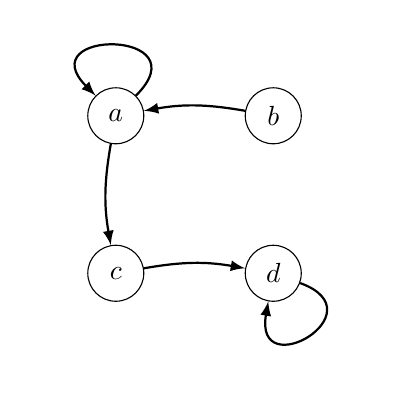
\begin{tikzpicture}
	
	\node[draw=black,circle,minimum width=0.28in] (a)  at (0,2) {$a$};
	\node[draw=black,circle,minimum width=0.28in] (b) at (2,2) {$b$};
	\node[draw=black,circle,minimum width=0.28in] (c) at (0,0) {$c$};
	\node[draw=black,circle,minimum width=0.28in] (d) at (2,0) {$d$};

	\path[->,>=latex,draw=black,thick ] (a) to[looseness=6] (a);
	\path[->,>=latex, draw=black,thick ] (b) to[looseness=1,in=10,out=170] (a);
	\path[->,>=latex,draw=black,   thick] (c) to[looseness=1,in=170,out=10] (d);
	\path[->,>=latex,draw=black,   thick] (a) to[looseness=1,in=100,out=260] (c);
	\path[->,>=latex,draw=black, thick] (d) to[out=340,in=260,looseness=6] (d);

\end{tikzpicture}
	
 
\end{document}




 


